\documentclass[a4paper,12pt]{article}
\usepackage{amsmath, amsthm}
\usepackage{datetime}
\usepackage{framed}
\usepackage{enumitem}
\usepackage{fancyref}
\usepackage{wrapfig}
\usepackage{pifont}
\usepackage{appendix}
\usepackage{caption}
\usepackage{xcolor}
\usepackage[stable]{footmisc}
\usepackage{multicol}
\usepackage{csquotes}
\usepackage{pdfpages}

\usepackage{amsthm}

\usepackage{amssymb}
\usepackage{amsfonts}
\usepackage{amsmath}
\usepackage{mathtools}

\usepackage{tikz}
\usepackage{pgf}
\usepgflibrary{fpu}
\usepackage{qtree}
\usetikzlibrary{angles,fit,arrows,calc,math,intersections,through,backgrounds,cd}
\usepackage{pgfplots}
\usepackage{tkz-euclide}

\usepackage{listings}
\lstset{
  basicstyle=\itshape,
  xleftmargin=3em,
  literate={->}{$\rightarrow$}{2}
           {α}{$\alpha$}{1}
           {δ}{$\delta$}{1}
}


\usepackage{csquotes}
\renewcommand{\mkbegdispquote}[2]{\itshape}

\newdateformat{nianyueri}{修订于 \THEYEAR 年 \THEMONTH 月 \THEDAY 日 }

\usepackage{xstring}
\usepackage{catchfile}
\CatchFileDef{\HEAD}{../.git/refs/heads/master}{}
\newcommand{\gitrevision}{%
  \StrLeft{\HEAD}{7}%
}

\usepackage{data/quiver}
\usepackage{data/circledsteps}
\usepackage[top=1in,bottom=1in,left=1in,right=1in]{geometry} % 用于设置页面布局
\usepackage{xeCJK} % 用于使用本地字体
\usepackage[super, square, sort&compress]{natbib} % 处理参考文献
\usepackage{titlesec, titletoc} % 设置章节标题及页眉页脚
%\usepackage{xCJKnumb} % 中英文数字转换
\usepackage{amssymb}
\usepackage{amsmath} % 在公式中用\text{文本}输入中文
\usepackage{diagbox}
\usepackage{multirow} % 表格中使用多行
\usepackage{booktabs} % 表格中使用\toprule等命令
\usepackage{rotating} % 使用sidewaystable环境旋转表格
\usepackage{tabularx}
\usepackage{graphicx} % 处理图片
\usepackage{footnote} % 增强的脚注功能,可添加表格脚注
\usepackage{threeparttable} % 添加真正的表格脚注,示例见README
\usepackage{hyperref} % 添加pdf书签

\usepackage{tikz}
\usetikzlibrary{shapes,arrows,shadows}

% 字体设置
\setmainfont{Times New Roman}
\setsansfont[Scale=MatchLowercase,Mapping=tex-text]{PT Sans}
\setmonofont[Scale=MatchLowercase]{PT Mono}
\setCJKmainfont[ItalicFont={Kaiti SC}, BoldFont={Heiti SC}]{Songti SC}
\setCJKsansfont{Heiti SC}
\setCJKmonofont{Songti SC}
% \setCJKmainfont[BoldFont={FZXiaoBiaoSong-B05S}]{Songti SC}
% \setCJKfamilyfont{kai}[BoldFont=Heiti SC]{Kaiti SC}
% \setCJKfamilyfont{song}[BoldFont=Heiti SC]{Songti SC}
% \setCJKfamilyfont{hei}[BoldFont=Heiti SC]{Heiti SC}
% \setCJKfamilyfont{fsong}[BoldFont=Heiti SC]{Songti SC}
% \newcommand{\kai}[1]{{\CJKfamily{kai}#1}}
% \newcommand{\hei}[1]{{\CJKfamily{hei}#1}}
% \setromanfont[Mapping=tex-text]{TeXGyrePagella}
% \setsansfont[Scale=MatchLowercase,Mapping=tex-text]{TeXGyrePagella}
% \setmonofont[Scale=MatchLowercase]{Courier New}
%%设置常用中文字号,方便调用
\newcommand{\erhao}{\fontsize{22pt}{\baselineskip}\selectfont}
\newcommand{\xiaoerhao}{\fontsize{18pt}{\baselineskip}\selectfont}
\newcommand{\sanhao}{\fontsize{16pt}{\baselineskip}\selectfont}
\newcommand{\xiaosanhao}{\fontsize{15pt}{\baselineskip}\selectfont}
\newcommand{\sihao}{\fontsize{14pt}{\baselineskip}\selectfont}
\newcommand{\xiaosihao}{\fontsize{12pt}{\baselineskip}\selectfont}
\newcommand{\wuhao}{\fontsize{10.5pt}{\baselineskip}\selectfont}
\newcommand{\xiaowuhao}{\fontsize{9pt}{\baselineskip}\selectfont}
\newcommand{\liuhao}{\fontsize{7.5pt}{\baselineskip}\selectfont}

% 章节标题显示方式及页眉页脚设置
% \item xCJKnumb是自己额外安装的包
% \item titleformat命令定义标题的形式
% \item titlespacing定义标题距左、上、下的距离
\titleformat{\section}{\raggedright\large\bfseries}{\thesection}{1em}{}
\titleformat{\subsection}{\raggedright\normalsize\bfseries}{\thesubsection}{1em}{}
\titlespacing{\section}{0pt}{*0}{*2}
\titlespacing{\subsection}{0pt}{*0}{*1}
% 由于默认的2em缩进不够,所以我手动调整了,但是在windows下似乎2.2就差不多了,或者是article中没有这个问题
\setlength{\parindent}{2.2em}

% 设置表格标题前后间距
\setlength{\abovecaptionskip}{0pt}
\setlength{\belowcaptionskip}{0pt}


\renewcommand{\refname}{\bfseries{参~考~文~献}} %将Reference改为参考文献(用于 article)
% \renewcommand{\bibname}{参~考~文~献} %将bibiography改为参考文献(用于 book)
\renewcommand{\baselinestretch}{1.38} %设置行间距
\renewcommand{\figurename}{\small\ttfamily 图}
\renewcommand{\tablename}{\small\ttfamily 表}


\usepackage{stmaryrd}
\usepackage{mathtools}
\usepackage{wasysym}
\usepackage{textcomp}
\usepackage{blindtext}
\usepackage{subfiles}

\newtheorem{problem}{问题}
\numberwithin{problem}{section}
\newtheorem{definition}{定义}
\numberwithin{definition}{section}
\newtheorem{lemma}{引理}
\numberwithin{lemma}{section}
\newtheorem{proposition}{命题}
\numberwithin{proposition}{section}
\newtheorem{theorem}{定理}
\numberwithin{theorem}{section}
\newtheorem{grammar}{文法}
\numberwithin{grammar}{section}
\newtheorem{program}{程序}
\numberwithin{program}{section}
\newtheorem{convention}{约定}
\numberwithin{convention}{section}
\newtheorem{corollary}{推论}
\numberwithin{corollary}{section}
\renewcommand*{\proofname}{证明}

\xeCJKsetwidth{‘’“”}{1em}

\title{有限、无限与想象力}
\date{\nianyueri\today}
\author{苑明理}

\begin{document}

\begingroup
\let\newpage\relax
\maketitle
\endgroup

\centerline{\rule{13cm}{0.4pt}}
\renewcommand{\contentsname}{\hfill\bfseries 目录\hfill}
\setcounter{tocdepth}{2}
\tableofcontents
\centerline{\rule{13cm}{0.4pt}}

\newpage

\section{语言模型的补全}

下面是展示语言模型补全能力的例子。

输入前文:\newline
\begin{displayquote}
艾达:你好,我是艾达,竭诚为您服务?有什么可以帮到你的吗?\newline
麦克:我们一起玩一个游戏可以吗?\newline
艾达:当然可以!你有什么想玩的游戏?\newline
麦克:我们一起猜谜语好吗?\newline
\end{displayquote}
输出补全:\newline
\begin{displayquote}
艾达:好啊!那我先来一个:“头上有角,身上有毛,叫声响亮,叫声可爱”。你猜是什么?\newline
\end{displayquote}

\section{补全是否图灵完备}

在上面的例子中,我们可以看到,语言模型的补全能力是非常强大的,它可以生成一个完整的对话。一个问题是,这个补全能力是否是图灵完备的呢?

我们知道组合子 $\iota$ 自己就已经图灵完全。因此,我们知道存在一种语言,它上面有图灵完备的函数。于是,问 LLM 的补全能力是否图灵完备,是一个完全合理的问题。

然而,在当前计算架构下,用有限精度浮点数计算神经网络,它的总状态数有限,从而无法模拟无限长纸带的所有状态,因此 LLM 的任何有限精度上的实现方案都不可能是图灵完全的。

\section{通用图灵机可否实现?}

图灵机的任何实现版本总状态数有限,从而无法模拟无限长纸带的所有状态,因此通用图灵机无法完整实现。

\section{机器能否数数?}

尝试用强化学习的思路,创造一个生存环境,智能体必须通过计数的方法来获得更优的选择,然后不限定智能体的策略的制定,如此从侧面去考察数的创造。

这种强化学习的思路,最终还是通过报酬或者激励的量化来驱动策略的搜索,也就是把数的创造问题化归为一个势能面上的寻优。这背后是一种\textbf{几何式的元数学}观点。

有限、无限的对立仍然会以别的形式出现,比如几何上的套笼—同样的游戏在更高一层上复现。

\section{“所有”指的是什么?}

我们怎么可能可以说“所有”?

\begin{displayquote}
我说:“所有的天鹅都是白色的”
\end{displayquote}

仔细分析这里的指代关系,就会发现,我说“所有”的时候,是基于我看到过的一些天鹅,然后声称了一个很强假设。

\begin{displayquote}
你听到我说的“所有的天鹅都是白色的”
\end{displayquote}

你的理解是基于你看到过的另外一些天鹅。

所以,“所有”的实际意义并不简单,它沿着空间展开,还面向未来展开。词语意义的飘移在这里甚至是必须的,否则无从谈论理解。

另一个例子
\begin{displayquote}
你上幼儿园的第一天,你会惊讶,因为你的一些“所有”的概念被推翻了,因为你以为“大家都爱你”的大家之前只有你的家人,幼儿园你发现了有一些人不爱你。
\end{displayquote}

人发明了全称的量词,但是对它的使用和解释是不断扩大的。小朋友是一个情况,成年人另外一种情况。但总的来说,这种不断变化的“全称”词语游戏,是人类想象力的体现。
只要这个游戏可以玩下去,它就能不断扩大游戏者体验到的世界。

\section{有限、无限与想象力}



\section{命题逻辑的蕴含}

\section{指称的秘密}

\section{一维的语言?}

\section{知识的极小曲面猜测}

Benacerraf 困境的一种表述

\begin{figure}[ht]
\centering
\begin{tikzpicture}
\draw (6, 2) node[inner sep=0] {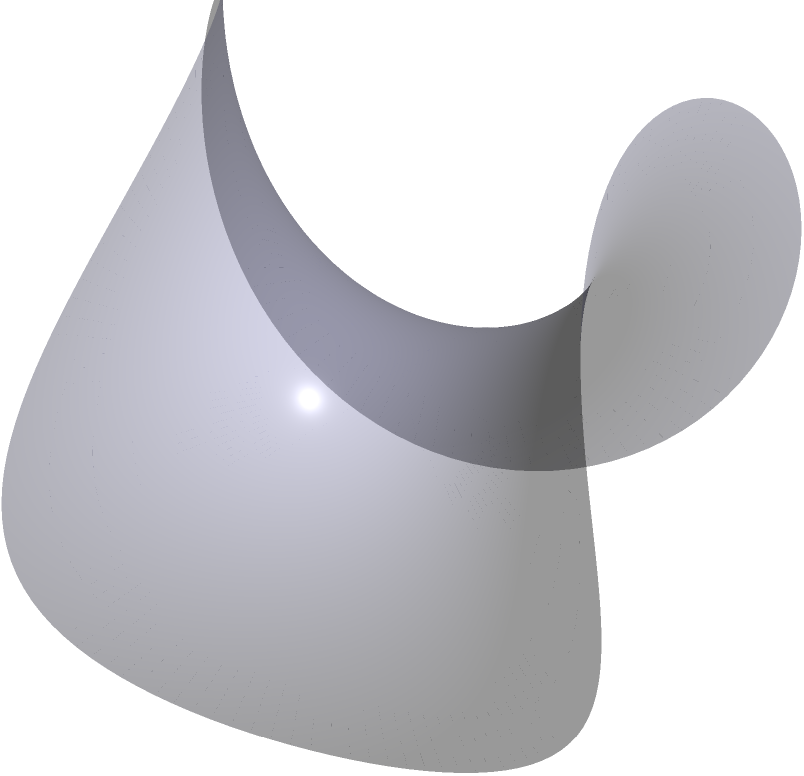
\includegraphics[width=4in]{images/ennepers.png}};
\node [anchor=225, black] at (9,6) {几何};
\node [anchor=225, black] at (9,-3) {分析};
\node [anchor=225, black] at (2,6) {计算};
\node [anchor=225, black] at (0,0) {学习};
\node [anchor=225, black] at (6,2) {算术表达式几何};
\end{tikzpicture}
\caption{知识的极小曲面}
\end{figure}

康德有论述“先天综合判断”,几何作为命题都呈现为“综合命题”,肥皂泡的几何式知识观有可能会暗合康德的理论。
这个知识观可以形式化为上面说的“过程与形式”的数学,而算术表达式几何就是这个“过程与形式”的数学的第一个例子。

\end{document}
